
\section{Modeling}

In the following we describe how you can create PCM-Models using the Workbench and how you can publish them to the server.

\subsection{Creating a new Model}

We assume that you have started the Workbench and the server. There are two ways to create a new model.
You can either use the File\textgreater\textgreater New menu or the New Icon.
Nevertheless, you always have to choose the type of the model to be created.

\subsection{Publish a Model}

If you create your diagrams in the Workbench and if you have a Processeditor Server running you can publish a model to the centralized repository (the server).
Therefore you have to do either, click on the Publish icon or use the menu item inside the file Menu.
Then you have to select a server and a name for the model.
In addition you can choose if you want to save the model as a new version of an existing one or as a new model.

\subsection{Fetch a Model}

If you work inside your Workbench you have to fetch Models from the server, in order to alter or view them.
To do so click on the Fetch icon or use the menu item inside the File menu.
You can now connect to a server.
After that you will see a tree with all diagrams and folders on the server model repository.
Choose the one you want to open.

\subsection{Modeling PCM-Fragments}

You can model a PCM Fragment by choosing the PCM Fragment type from the context menu. Now you can add nodes by clicking right on the canvas. You can choose from Start Events, Activities, Gateways, End Events and Data Objects.

If you want to use the created model for the execution in the engine you have to be aware of the following constraints:

\begin{itemize}
\item Every fragment must contain exactly one start and end event
\item All Events must be blank
\item The activities must be either blank, Sending Mail Task or Service Task
\item The Gateways must be exclusive or parallel ones
\end{itemize}

\noindent
\textbf{Referring an Activity From Another Fragment}

\noindent
If you want to refer an activity from another Fragment you have to do the following steps.
\begin{enumerate}
\item The task in the other fragment has to be marked as global (right click on activity, properties, global).
\item This fragment has to be published on a server.
\item Make a right click choose Copy and Refer Task. Select the Fragment and the Task to be copied.
\end{enumerate} 
The task will be added to the current model.
\noindent
You can add edges either by dragging a new node from the context menu of the previous node or by pressing and holding the right button.

\subsection{Modeling a Data Model}

If you want to create a Data Model for the Data Objects in your PCM Process you have to create a new Domain Model. Again, if you want to use this model from within the JEngine you have to publish it and you should at most create one Root Class.
Right click "Edit Attributes" Allows you to add and remove attributes for each class.
You can create relations between data classes using an Aggregation by pressing and holding the right mouse button.

\subsection{Modeling a PCM Scenario}

A PCM Scenario holds the whole Process, therefore it needs information about all fragments, the data objects and their relation to data classes. Hence, a couple of steps are necessary.
\begin{enumerate}
\item \textbf{Adding Fragments}.
First of all you have to add new Fragments. You can do this by using the plugin "Add Fragments" from within the process's contexts menu. Now you can connect to a server and select a number of Fragments from the right side, which should be added to the scenario.
\item \textbf{Define a Domain-Model}.
Every Scenario needs an Domain Model, therefore go to the properties of the model and paste the URL of the domain model into the domainModelURL Property. The server address must be the same as specified in the configuration class of the JEngine. This means the default URL would be \url{http://localhost:1205/models/<domainModelId>.pm}.
\item \textbf{Map Data Objects to Data Classes}.
Every Data Object needs one Data Class.
Hence, you must assign one.
You can do this by editing the properties (figure \ref{pic:propdo}). If you want to execute the scenario you have to make sure, that the selected data class is in the model assigned to the PCM Scenario.
\item \textbf{Define a Termination Condition}.
A Scenario needs a clear termination condition. You can define it inside the properties menu (figure \ref{pic:propscen}) of the process. There type the name of exactly one data object int the field and the state surrounded by [ ] in the state field.
\end{enumerate}
\begin{figure}[h!]
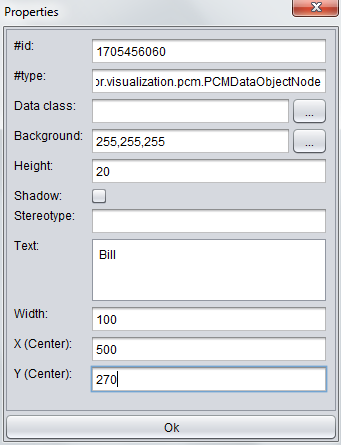
\includegraphics[height=0.4\textheight]{graphics/dataNodeProperties.png}
\caption{Properties of a Data Object Node}
\label{pic:propdo}
\end{figure}

\begin{figure}[h!]
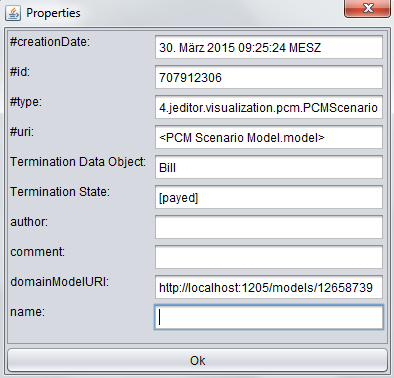
\includegraphics[height=0.4\textheight]{graphics/scenarioProperties.png}
\caption{Properties of a PCM Scenario}
\label{pic:propscen}
\end{figure}
\noindent
Make sure to publish the scenario, the domain model and all fragments to the process repository.